\documentclass[reqno, 12pt]{amsart}

\usepackage{amssymb, amsmath, amsthm, enumerate, mathtools, graphicx, enumitem, tikz, color, soul, bbm, verbatim, parskip, multicol}
\usepackage[margin=1 in]{geometry}
\usepackage[mathscr]{euscript}
\usepackage[urlcolor=blue,colorlinks=true]{hyperref}
\setlist[itemize]{noitemsep, topsep=0pt, parsep=0pt, partopsep=0pt}
\allowdisplaybreaks

\newcommand{\R}{\mathbb R}
\newcommand{\proj}{\operatorname{proj}}

\usepackage{mdframed}
\newmdenv[
  linewidth=1pt,
  linecolor=black,
  topline=true,
  bottomline=true,
  leftline=true,
  rightline=true,
  innertopmargin=10pt,
  innerbottommargin=10pt,
  innerleftmargin=10pt,
  innerrightmargin=10pt
]{answerbox}

\usepackage{pgfplots}
\pgfplotsset{compat=1.18}
\usepgfplotslibrary{fillbetween}


\pagestyle{plain}


\begin{document}

\begin{center}
  {\bf MATH 231-01: Homework Assignment 7}\\~\\
  27 October 2025\\~\\~\\~\\~\\~\\
\end{center}

{\bf Due:} 3 November 2025 by 10:00pm Eastern time, submitted on Moodle as a single PDF.~\\


{\bf Instructions:} Write your solutions on the following pages. If you need more space, you may add pages, but make sure they are in order and label the problem number(s) clearly. You should attempt each problem on scrap paper first, before writing your solution here. Excessively messy or illegible work will not be graded. You must show your work/reasoning to receive credit. You do not need to include every minute detail; however the process by which you reached your answer should be evident. You may work with other students, but please write your solutions in your own words.

~\\~\\~\\~\\~\\
{\bf Name:} Sean Balbale

~\\
{\bf Score:}

\newpage
\begin{itemize}
  \item[1.] Let $R$ be the region bounded by the parabola $x = y^2$ and the line $y=x-2$. Evaluate the double integral $\displaystyle\iint_R xydA$.
    \newline

    \begin{answerbox}
      \begin{enumerate}
        \item First, we need to find the points of intersection between the parabola and the line. Setting $x = y^2$ equal to $y = x - 2$, we have:
          \[y^2 = y + 2 \implies y^2 - y - 2 = 0\]
          Factoring the quadratic, we get:
          \[(y - 2)(y + 1) = 0\]
          Thus, the points of intersection are $y = 2$ and $y = -1$. Substituting these back into either equation to find the corresponding $x$ values, we get:
          \[x = 2^2 = 4 \quad \text{and} \quad x = (-1)^2 = 1\]
          Therefore, the points of intersection are $(4, 2)$ and $(1, -1)$.
        \item Next, we set up the double integral. The region $R$ can be described in terms of $x$ and $y$ as follows:
          \[-1 \leq y \leq 2\]
          For each fixed $y$, $x$ ranges from the parabola to the line:
          \[y^2 \leq x \leq y + 2\]
          Thus, the double integral becomes:
          \[\iint_R xy \, dA = \int_{y=-1}^{y=2} \int_{x=y^2}^{y+2} xy \, dx \, dy\]
        \item Now, we evaluate the inner integral:
          \begin{align*}
            \int_{x=y^2}^{y+2} xy \, dx &= y \int_{x=y^2}^{y+2} x \, dx \\
            &= y \left[ \frac{x^2}{2} \right]_{x=y^2}^{y+2} \\
            &= y \left( \frac{(y+2)^2}{2} - \frac{(y^2)^2}{2} \right) \\
            &= y \left( \frac{y^2 + 4y + 4 - y^4}{2} \right) \\
            &= \frac{y(y^2 + 4y + 4 - y^4)}{2} \\
            &= \frac{y^3 + 4y^2 + 4y - y^5}{2}
          \end{align*}
        \item Finally, we evaluate the outer integral:
          \[\int_{y=-1}^{y=2} \frac{y^3 + 4y^2 + 4y - y^5}{2} \, dy = \frac{1}{2} \int_{y=-1}^{y=2} ( y^3 + 4y^2 + 4y - y^5 ) \, dy\]
          Evaluating this integral, we find:
          \[\frac{1}{2} \left[ \frac{y^4}{4} + \frac{4y^3}{3} + 2y^2 - \frac{y^6}{6} \right]_{y=-1}^{y=2}\]
          Calculating the values at the bounds:
          \[\text{At } y=2: \frac{16}{4} + \frac{32}{3} + 8 - \frac{64}{6} = 4 + \frac{32}{3} + 8 - \frac{32}{3} = 12\]
          \[\text{At } y=-1: \frac{1}{4} - \frac{4}{3} + 2 - \frac{1}{6} = \frac{3}{12} - \frac{16}{12} + \frac{24}{12} - \frac{2}{12} = \frac{9}{12} = \frac{3}{4}\]
          Therefore, the value of the integral is:
          \[\frac{1}{2} (12 - \frac{3}{4}) = \frac{1}{2} \left( \frac{48}{4} - \frac{3}{4} \right) = \frac{1}{2} \left( \frac{45}{4} \right) = \frac{45}{8}\]
          Thus, the value of the double integral is $\boxed{\frac{45}{8}}$.
      \end{enumerate}
    \end{answerbox}
    \vspace{0.5 in}

  \item[2.] Let $R$ be the triangular region with vertices $(0,0)$, $(1,1)$, and $(-1,2)$. Evaluate the double integral $\displaystyle\iint_R xy dA$.
    \newline

    \begin{answerbox}
      \begin{enumerate}
        \item First, we need to determine the equations of the lines that form the sides of the triangle. The vertices are $(0,0)$, $(1,1)$, and $(-1,2)$. The equations of the lines are:
          \begin{itemize}
            \item Line from $(0,0)$ to $(1,1)$: $y = x$
            \item Line from $(0,0)$ to $(-1,2)$: $y = -2x$
            \item Line from $(1,1)$ to $(-1,2)$: $y = -\frac{1}{2}x + \frac{3}{2}$
          \end{itemize}
        \item We must find the bounds for $x$ and $y$. The triangle can be split into two regions based on $y$:
          \begin{itemize}
            \item For $-1 \leq x \leq 0$, $y$ ranges from $-2x$ to $-\frac{1}{2}x + \frac{3}{2}$.
            \item For $0 \leq x \leq 1$, $y$ ranges from $x$ to $-\frac{1}{2}x + \frac{3}{2}$.
          \end{itemize}
        \item Thus, we can set up the double integral as follows:
          \[\iint_R xy \, dA = \int_{x=-1}^{x=0} \int_{y=-2x}^{y=-\frac{1}{2}x + \frac{3}{2}} xy \, dy \, dx + \int_{x=0}^{x=1} \int_{y=x}^{y=-\frac{1}{2}x + \frac{3}{2}} xy \, dy \, dx\]
        \item Now, we evaluate the first integral:
          \begin{align*}
            \int_{x=-1}^{x=0} \int_{y=-2x}^{y=-\frac{1}{2}x + \frac{3}{2}} xy \, dy \, dx &= \int_{x=-1}^{x=0} x \left[ \frac{y^2}{2} \right]_{y=-2x}^{y=-\frac{1}{2}x + \frac{3}{2}} \, dx \\
            &= \int_{x=-1}^{x=0} \frac{x}{2} \left[ \left(-\frac{1}{2}x + \frac{3}{2}\right)^2 - (-2x)^2 \right] \, dx \\
            &= \int_{x=-1}^{x=0} \frac{x}{2} \left[ \left(\frac{1}{4}x^2 - \frac{3}{2}x + \frac{9}{4}\right) - 4x^2 \right] \, dx \\
            &= \int_{x=-1}^{x=0} \frac{x}{2} \left[ -\frac{15}{4}x^2 - \frac{3}{2}x + \frac{9}{4} \right] \, dx \\
            &= \int_{x=-1}^{x=0} \left( -\frac{15}{8}x^3 - \frac{3}{4}x^2 + \frac{9}{8}x \right) \, dx \\
            &= \left[ -\frac{15}{32}x^4 - \frac{1}{4}x^3 + \frac{9}{16}x^2 \right]_{x=-1}^{x=0} \\
            &= (0) - \left( -\frac{15}{32} + \frac{1}{4} + \frac{9}{16} \right) \\
            &= - \left( \frac{-15 + 8 + 18}{32} \right) = -\frac{11}{32}
          \end{align*}
        \item Next, we evaluate the second integral:
          \begin{align*}
            \int_{x=0}^{x=1} \int_{y=x}^{y=-\frac{1}{2}x + \frac{3}{2}} xy \, dy \, dx &= \int_{x=0}^{x=1} x \left[ \frac{y^2}{2} \right]_{y=x}^{y=-\frac{1}{2}x + \frac{3}{2}} \, dx \\
            &= \int_{x=0}^{x=1} \frac{x}{2} \left[ \left(-\frac{1}{2}x + \frac{3}{2}\right)^2 - (x)^2 \right] \, dx \\
            &= \int_{x=0}^{x=1} \frac{x}{2} \left[ \left(\frac{1}{4}x^2 - \frac{3}{2}x + \frac{9}{4}\right) - x^2 \right] \, dx \\
            &= \int_{x=0}^{x=1} \frac{x}{2} \left[ -\frac{3}{4}x^2 - \frac{3}{2}x + \frac{9}{4} \right] \, dx \\
            &= \int_{x=0}^{x=1} \left( -\frac{3}{8}x^3 - \frac{3}{4}x^2 + \frac{9}{8}x \right) \, dx \\
            &= \left[ -\frac{3}{32}x^4 - \frac{1}{4}x^3 + \frac{9}{16}x^2 \right]_{x=0}^{x=1} \\
            &= \left( -\frac{3}{32} - \frac{1}{4} + \frac{9}{16} \right) - (0) \\
            &= \frac{-3 - 8 + 18}{32} = \frac{7}{32}
          \end{align*}
        \item Finally, we add the results of the two integrals:
          \begin{align*}
            \iint_R xy \, dA &= -\frac{11}{32} + \frac{7}{32} = -\frac{4}{32} = -\frac{1}{8}
          \end{align*}
          Thus, the value of the double integral is $\boxed{-\frac{1}{8}}$.
      \end{enumerate}
    \end{answerbox}
    \vspace{0.5 in}
    \newpage
  \item[3.] Evaluate the iterated integral $\displaystyle\int_0^2\int_0^{\sqrt{4-x^2}} \sqrt{x^2+y^2} dydx$.
    \newline

    \begin{answerbox}
      \begin{enumerate}
        \item First, we convert the given integral to polar coordinates. Graphing the region we get:
          \begin{center}
            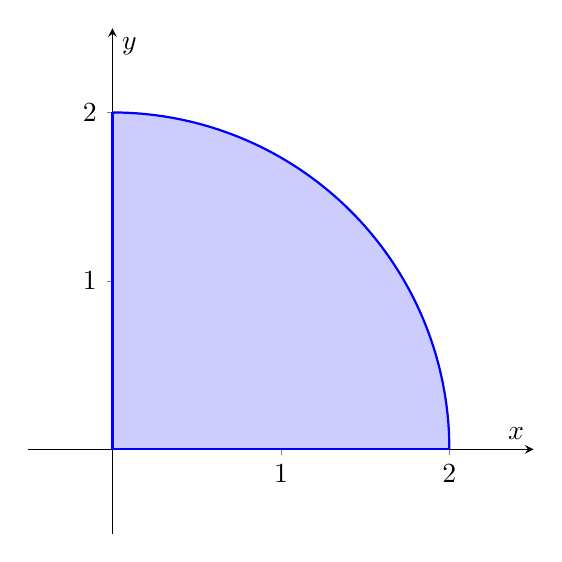
\begin{tikzpicture}[scale=1]
              \begin{axis}[
                  axis lines = middle,
                  xlabel = $x$,
                  ylabel = $y$,
                  xtick={0,1,2},
                  ytick={0,1,2},
                  xmin=-0.5, xmax=2.5,
                  ymin=-0.5, ymax=2.5,
                  domain=0:2,
                  samples=1000,
                  width=8cm,
                  height=8cm,
                ]
                % Quarter circle
                \addplot [name path=A, thick, blue] {sqrt(4 - x^2)};
                % x-axis
                \addplot [name path=B, thick, blue] {0};
                % y-axis boundary
                \addplot [thick, blue] coordinates {(0,0) (0,2)};
                % Fill the area
                \addplot [fill=blue!20] fill between [of=A and B, soft clip={domain=0:2}];
              \end{axis}
            \end{tikzpicture}
          \end{center}
          The region of integration is bounded by $x=0$ to $x=2$ and $y=0$ to $y=\sqrt{4-x^2}$, which describes a quarter circle of radius 2 in the first quadrant. In polar coordinates, we have:
          \[x = r\cos\theta, \quad y = r\sin\theta, \quad dA = r \, dr \, d\theta\]
          The limits for $r$ are from $0$ to $2$, and for $\theta$ from $0$ to $\frac{\pi}{2}$. The integrand $\sqrt{x^2 + y^2}$ becomes $\sqrt{r^2} = r$. Thus, the integral in polar coordinates is:
          \[\int_{\theta=0}^{\frac{\pi}{2}} \int_{r=0}^{2} r \cdot r \, dr \, d\theta = \int_{0}^{\frac{\pi}{2}} \int_{0}^{2} r^2 \, dr \, d\theta\]
        \item Next, we evaluate the inner integral:
          \begin{align*}
            \int_{0}^{2} r^2 \, dr &= \left[ \frac{r^3}{3} \right]_{0}^{2} = \frac{8}{3}
          \end{align*}
        \item Now, we evaluate the outer integral:
          \begin{align*}
            \int_{0}^{\frac{\pi}{2}} \frac{8}{3} \, d\theta &= \frac{8}{3} \left[ \theta \right]_{0}^{\frac{\pi}{2}} = \frac{8}{3} \cdot \frac{\pi}{2} = \frac{4\pi}{3}
          \end{align*}
          Thus, the value of the iterated integral is $\boxed{\frac{4\pi}{3}}$.
      \end{enumerate}
    \end{answerbox}
    \vspace{0.5 in}
    \newpage
  \item[4.] Let $R$ be the lamina occupying the region bounded by the parabolas $x=y^2$ and $y = x^2$. Assuming $R$ has density given by $\rho(x,y) = \sqrt{x}$, find its center of mass.
    \newline

    \begin{answerbox}
      \begin{enumerate}
        \item First, we need to find the points of intersection between the parabolas $x = y^2$ and $y = x^2$. Setting $x = y^2$ equal to $y = x^2$, we have:
          \[y^2 = (y^2)^2 \implies y^2 = y^4 \implies y^4 - y^2 = 0 \implies y^2(y^2 - 1) = 0\]
          Thus, the points of intersection are $y = 0$, $y = 1$, and $y = -1$. Substituting these back into either equation to find the corresponding $x$ values, we get:
          \[x = 0^2 = 0, \quad x = 1^2 = 1, \quad x = (-1)^2 = 1\]
          Therefore, the points of intersection are $(0,0)$ and $(1,1)$ (noting that both curves pass through the origin and meet at $(1,1)$).
        \item Next, we set up the double integral for the mass $M$ of the lamina:
          \[M = \iint_R \rho(x,y) \, dA = \iint_R \sqrt{x} \, dA\]
          The region $R$ can be described as a Type I region in terms of $x$ and $y$ as follows:
          \[0 \leq x \leq 1\]
          For each fixed $x$, $y$ ranges from the lower parabola $y = x^2$ to the upper parabola $y = \sqrt{x}$:
          \[x^2 \leq y \leq \sqrt{x}\]
          Thus, the double integral for mass becomes:
          \[M = \int_{x=0}^{1} \int_{y=x^2}^{\sqrt{x}} \sqrt{x} \, dy \, dx\]
          Evaluating the inner integral:
          \begin{align*}
            \int_{y=x^2}^{\sqrt{x}} \sqrt{x} \, dy &= \sqrt{x} [y]_{y=x^2}^{\sqrt{x}} = \sqrt{x} (\sqrt{x} - x^2) = x - x^{5/2}
          \end{align*}
          Now, evaluating the outer integral:
          \begin{align*}
            M &= \int_{0}^{1} (x - x^{5/2}) \, dx = \left[ \frac{x^2}{2} - \frac{2x^{7/2}}{7} \right]_{0}^{1} = \frac{1}{2} - \frac{2}{7} = \frac{7-4}{14} = \frac{3}{14}
          \end{align*}
        \item Next, we find the moment $M_x$:
          \[M_x = \iint_R y \rho(x,y) \, dA = \int_{0}^{1} \int_{x^2}^{\sqrt{x}} y \sqrt{x} \, dy \, dx\]
          Evaluating the inner integral:
          \begin{align*}
            \int_{x^2}^{\sqrt{x}} y \sqrt{x} \, dy &= \sqrt{x} \left[ \frac{y^2}{2} \right]_{y=x^2}^{\sqrt{x}} = \frac{\sqrt{x}}{2} \left[ (\sqrt{x})^2 - (x^2)^2 \right] \\
            &= \frac{\sqrt{x}}{2} (x - x^4) = \frac{1}{2}(x^{3/2} - x^{9/2})
          \end{align*}
          Now, evaluating the outer integral:
          \begin{align*}
            M_x &= \int_{0}^{1} \frac{1}{2}(x^{3/2} - x^{9/2}) \, dx = \frac{1}{2} \left[ \frac{2x^{5/2}}{5} - \frac{2x^{11/2}}{11} \right]_{0}^{1} \\
            &= \frac{1}{2} \left( \frac{2}{5} - \frac{2}{11} \right) = \frac{1}{2} \left( \frac{22 - 10}{55} \right) = \frac{1}{2} \cdot \frac{12}{55} = \frac{6}{55}
          \end{align*}
        \item Similarly, for $M_y$, we have:
          \[M_y = \iint_R x \rho(x,y) \, dA = \int_{0}^{1} \int_{x^2}^{\sqrt{x}} x \sqrt{x} \, dy \, dx = \int_{0}^{1} \int_{x^2}^{\sqrt{x}} x^{3/2} \, dy \, dx\]
          Evaluating the inner integral:
          \begin{align*}
            \int_{x^2}^{\sqrt{x}} x^{3/2} \, dy &= x^{3/2} [y]_{y=x^2}^{\sqrt{x}} = x^{3/2} (\sqrt{x} - x^2) = x^2 - x^{7/2}
          \end{align*}
          Now, evaluating the outer integral:
          \begin{align*}
            M_y &= \int_{0}^{1} (x^2 - x^{7/2}) \, dx = \left[ \frac{x^3}{3} - \frac{2x^{9/2}}{9} \right]_{0}^{1} = \frac{1}{3} - \frac{2}{9} = \frac{3-2}{9} = \frac{1}{9}
          \end{align*}
        \item Finally, the coordinates of the center of mass $(\bar{x}, \bar{y})$ are given by:
          \[
            \bar{x} = \frac{M_y}{M} = \frac{1/9}{3/14} = \frac{1}{9} \cdot \frac{14}{3} = \frac{14}{27}, \quad \bar{y} = \frac{M_x}{M} = \frac{6/55}{3/14} = \frac{6}{55} \cdot \frac{14}{3} = \frac{28}{55}
          \]
          Therefore, the center of mass of the lamina is $\boxed{\left( \frac{14}{27}, \frac{28}{55} \right)}$.
      \end{enumerate}
    \end{answerbox}
    \vspace{0.5 in}
    
  \item[5.] In this exercise, you will determine the value of the integral
    \begin{align*}
      I = \int_{-\infty}^\infty e^{-x^2}dx.
    \end{align*}
    To get you started, observe that
    \begin{align*}
      I^2 = \Big(\int_{-\infty}^\infty e^{-x^2}dx\Big)\Big(\int_{-\infty}^\infty e^{-y^2}dy\Big) = \int_{-\infty}^\infty\int_{-\infty}^\infty e^{-(x^2+y^2)}dxdy.
    \end{align*}

    \begin{itemize}
      \item[(a)] Show that $\displaystyle\int_{-\infty}^\infty\int_{-\infty}^\infty e^{-(x^2+y^2)}dxdy = \int_0^{2\pi}\int_0^\infty e^{-r^2}rdrd\theta$.
        \newline

        \begin{answerbox}
          To convert the double integral from Cartesian coordinates to polar coordinates, we use the transformations:
          \[x = r\cos\theta, \quad y = r\sin\theta, \quad dA = r \, dr \, d\theta\]
          The integrand $e^{-(x^2 + y^2)}$ becomes $e^{-r^2}$ in polar coordinates since:
          \[x^2 + y^2 = r^2(\cos^2\theta + \sin^2\theta) = r^2\]
          The limits for $r$ are from $0$ to $\infty$, and for $\theta$ from $0$ to $2\pi$. Thus, the double integral in polar coordinates is:
          \[\int_{0}^{2\pi} \int_{0}^{\infty} e^{-r^2} r \, dr \, d\theta\]
          Therefore, we have shown that:
          \[\int_{-\infty}^\infty\int_{-\infty}^\infty e^{-(x^2+y^2)}dxdy = \int_0^{2\pi}\int_0^\infty e^{-r^2}rdrd\theta\]
        \end{answerbox}
        \vspace{0.5 in}
      \item[(b)] Evaluate the iterated integral $\displaystyle\int_0^{2\pi}\int_0^\infty e^{-r^2}rdrd\theta$ and state the value of $I$.
        \newline

        \begin{answerbox}
          To evaluate the iterated integral, we first compute the inner integral:
          \begin{align*}
            \int_0^\infty e^{-r^2} r \, dr
          \end{align*}
          We can use the substitution $u = r^2$, which gives $du = 2r \, dr$ or $r \, dr = \frac{du}{2}$. Changing the limits accordingly, when $r = 0$, $u = 0$, and when $r \to \infty$, $u \to \infty$. Thus,
          \begin{align*}
            \int_0^\infty e^{-r^2} r \, dr &= \int_0^\infty e^{-u} \frac{du}{2} = \frac{1}{2} \int_0^\infty e^{-u} \, du \\
            &= \frac{1}{2} \left[ -e^{-u} \right]_0^\infty = \frac{1}{2} (0 + 1) = \frac{1}{2}
          \end{align*}
          Now, we evaluate the outer integral:
          \begin{align*}
            \int_0^{2\pi} \frac{1}{2} \, d\theta &= \frac{1}{2} \left[ \theta \right]_0^{2\pi} = \frac{1}{2} (2\pi - 0) = \pi
          \end{align*}
          Therefore, we have:
          \[\int_0^{2\pi}\int_0^\infty e^{-r^2}rdrd\theta = \pi\]
          Since we established earlier that $I^2 = \int_{-\infty}^\infty\int_{-\infty}^\infty e^{-(x^2+y^2)}dxdy$, we have:
          \[I^2 = \pi \implies I = \sqrt{\pi}\]
          Thus, the value of the integral $I$ is $\boxed{\sqrt{\pi}}$.
        \end{answerbox}
        \vspace{0.5 in}
    \end{itemize}
\end{itemize}
\end{document}
